\documentclass[xcolor=table]{beamer}

% Get settings
\usepackage{mybeamer}

% Formalia
\title{Support decision system for diagnosing rare diseases using vector space model and medical text mining}
\subtitle{DIKU Bachelorprojekt 2009 -- 2010\\{\tiny Henrik G. Jensen, Michael Andersen}}
\author{}
\date{Vinter 2010}

\begin{document}

\begin{frame}
    \titlepage
\end{frame}

\section[Oversigt]{}
\begin{frame}

    \frametitle{\ }

    \begin{itemize}
        \item Kort introduktion til det gyldne snit
        \item Kan vi finde brug af det gyldne snit i malerkunsten?
        \item Resultater
    \end{itemize}

\end{frame}

% Begin actual slides
% 1
\section{Det gyldne snit}
\subsection*{}

\begin{frame}

    \frametitle{Division in Extreme and Mean Ratios}

    \begin{quote}
        ``A straight line is said to have been cut in extreme
        and mean ratio when, as the whole line is to the greater
        segment, so is the greater to the less.'' - Euklid
    \end{quote}

    \begin{figure}[!h]
        \centering
        \begin{picture}(240,5)
            \put(0, 10){$A$}
            \put(3, -5){\line(0, 1){10}}

            \put(75, 10){$\varphi$}

            \put(144, 10){$C$}
            \put(147, -4){\line(0, 1){8}}

            \put(192, 10){$1$}

            \put(233, 10){$B$}
            \put(236, -5){\line(0, 1){10}}

            \put(3, 0){\line(1, 0){233}}
        \end{picture}
    \end{figure}

    \begin{block}{Historie}

        \begin{itemize}
            \item Kendt af Euklid ca. 300 f. Kr. som \emph{DEMR}.
            \item Luca Pacioli kaldte det for \emph{De Divina Proportione} i 1509.
            \item Navngivet \emph{der Goldener Schnitt} af Martin Ohm i 1835.
        \end{itemize}

    \end{block}

\end{frame}

% 2

\subsection*{}
\begin{frame}

    \frametitle{Matematisk definition}

    Fra Euklids beskrivelse får vi

    \[
        \varphi = \frac{A\ C}{C\ B} = \frac{A\ B}{A\ C}
    \]
    \[
        \varphi = \frac{\varphi + 1}{\varphi}
    \]
    hvilket kan omskrives til en andengradsligning. Løsningen er det vi kalder det gyldne snit.

    \[
        \varphi^2 - \varphi -1 = 0
    \]
    \[
        \varPhi = \frac{\sqrt{5} - 1}{2}, \varphi = \frac{\sqrt{5} + 1}{2}
    \]
    \[
        \varPhi = 0.6180~3398~\ldots, \varphi = 1.6180~3398~\ldots
    \]

\end{frame}

\subsection*{}
\begin{frame}

    \frametitle{Hvor findes det gyldne snit?}

    \begin{block}{Hypoteser}

        Det gyldne snit er:

        \begin{itemize}
            \item <1> at finde i naturen.
            \item <1> specielt æstetisk tiltalende.
            \item <1> anvendt i arkitektur.
            \item <1-2> brugt i kompositionen af mange malerier.
        \end{itemize}

    \end{block}

    \visible<2>{
        \centering\vspace{1em}
        \textbf{Vi vil gerne undersøge om der fines noget \emph{interessant} i det gyldne snit i malerier.}
    }

\end{frame}

\section{Det gyldne snit i malerkunsten}

\subsection*{}
\begin{frame}

    \frametitle{Findes det gyldne snit i malerkunsten?}

    At undersøge om der findes noget interessant i det gyldne snit,
    rejser nogle vigtige spørgsmål.

    \hspace{8em}

    \begin{block}{Spørgsmål}

        \begin{itemize}
            \item Hvad er \emph{interessant} i maleriet?
            \item Hvor \emph{er} det gyldne snit i et maleri?
            \item Hvornår \emph{findes} noget i det gyldne snit?
        \end{itemize}

    \end{block}

\end{frame}

\subsection*{}
\begin{frame}

    \frametitle{Interessante regioner}

    \begin{block}{Hvad er en interessant region?}
        \begin{itemize}
            \item Meget svært at afgøre generelt.
            \item Afhænger af konteksten.
            \item Subjektivt.
        \end{itemize}
    \end{block}

    \begin{center}
        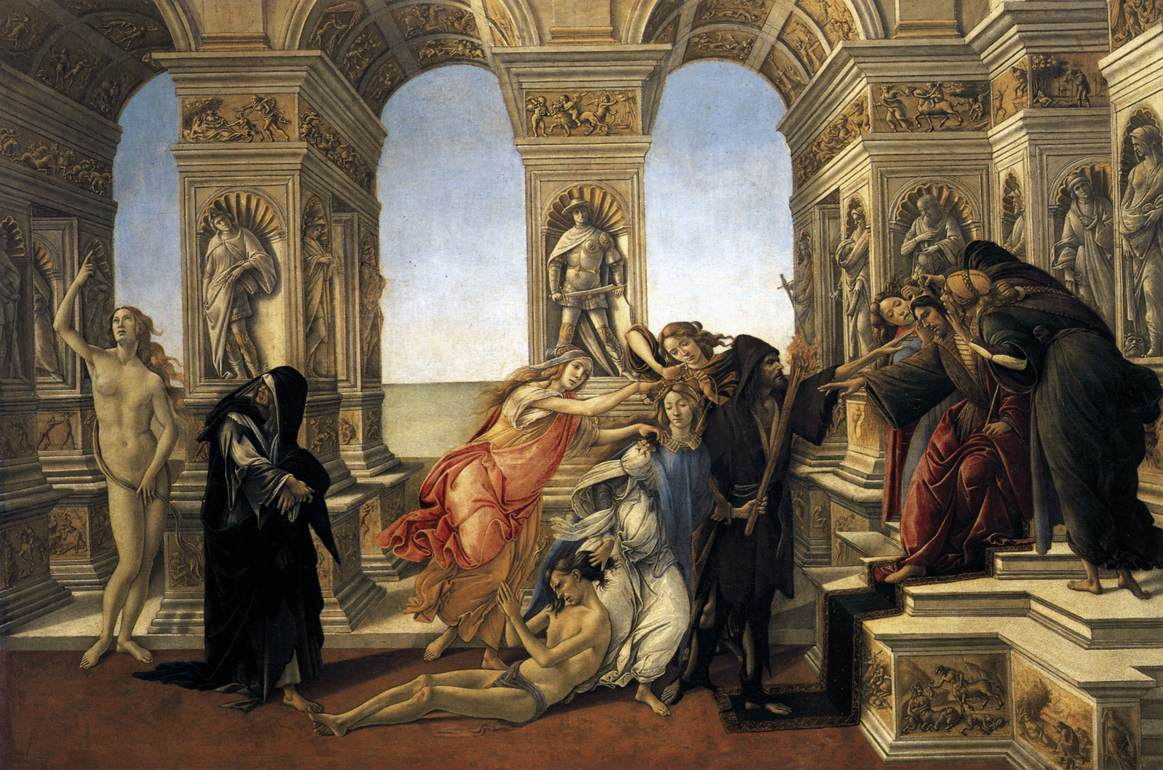
\includegraphics[width=0.67\textwidth]{billeder/10calumn.jpg}
    \end{center}

\end{frame}

\begin{frame}

    \frametitle{Hvad er interessant her?}

    \begin{center}
        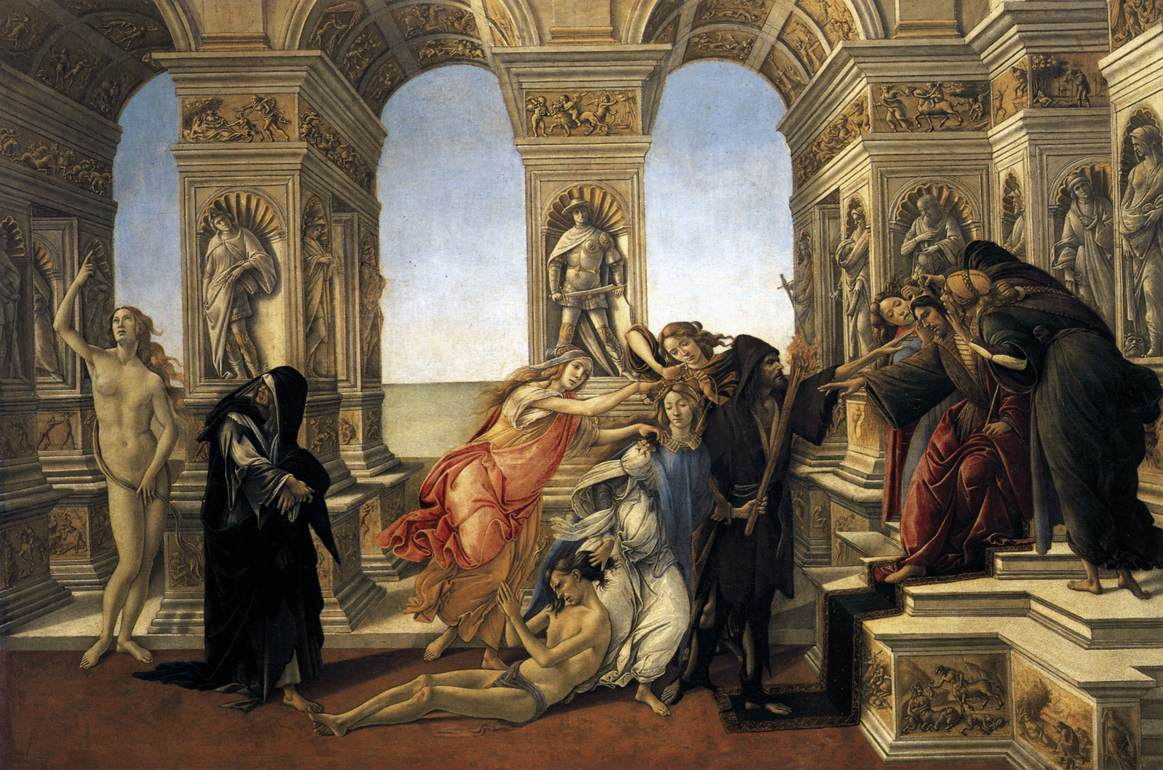
\includegraphics[width=1.00\textwidth]{billeder/10calumn.jpg}
    \end{center}

\end{frame}

\subsection*{}
\begin{frame}

    \frametitle{Interessante regioner}

    Vi har meget forskelige malerier, og det er meget svært, at fastsætte noget globalt mål, for
    hvad der er interessant i disse.

    \begin{definition}
        En \textbf{region} er en sammenhængende, ensfarvet gruppe pixels i
        et billede.
    \end{definition}

    \begin{definition}
        For at en region kan betegnes som \textbf{interessant}, skal den
        \begin{itemize}
            \item have et areal større end en tærskelværdi, der sættes i
                forhold til billedets størrelse
            \item have en masse større end en tærskelværdi, der ligeledes,
                sættes i forhold til billedets størrelse,
        \end{itemize}
    \end{definition}

\end{frame}

\subsection*{}
\begin{frame}

    \frametitle{Opdeling efter det gyldne snit}

    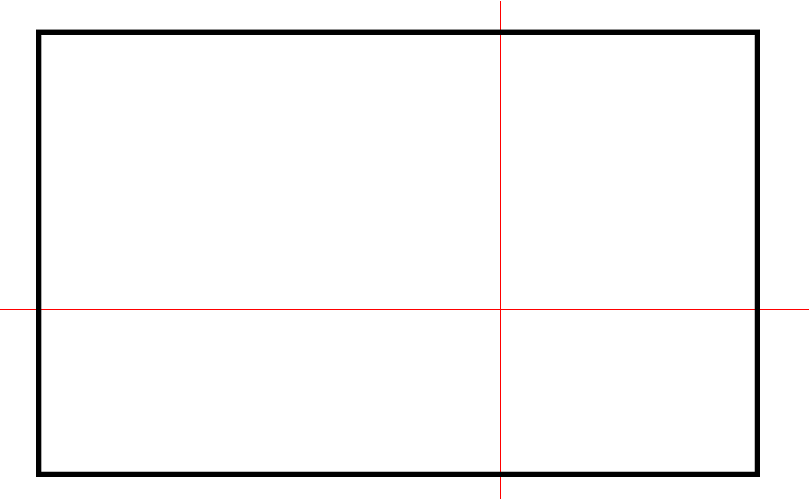
\includegraphics[width=\textwidth]{billeder/scan_direction.png}

\end{frame}

\subsection*{}
\begin{frame}

    \frametitle{Udtrækning af regioner}

    \only<1>{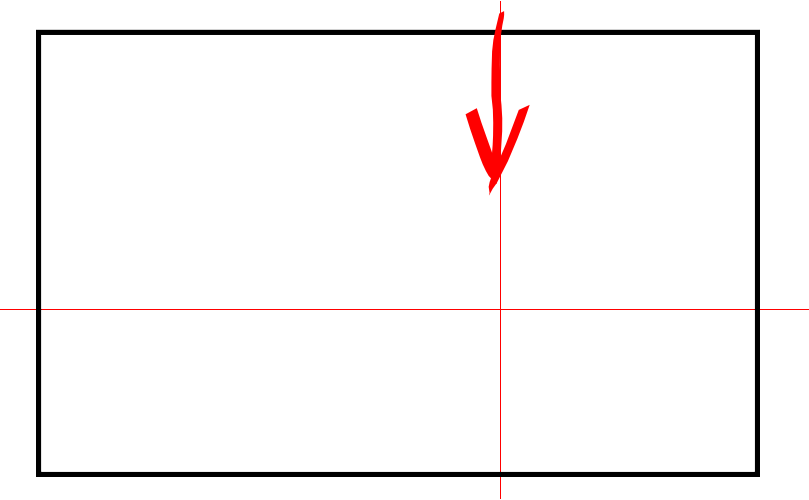
\includegraphics[width=\textwidth]{billeder/scan_direction_down.png}}
    \only<2>{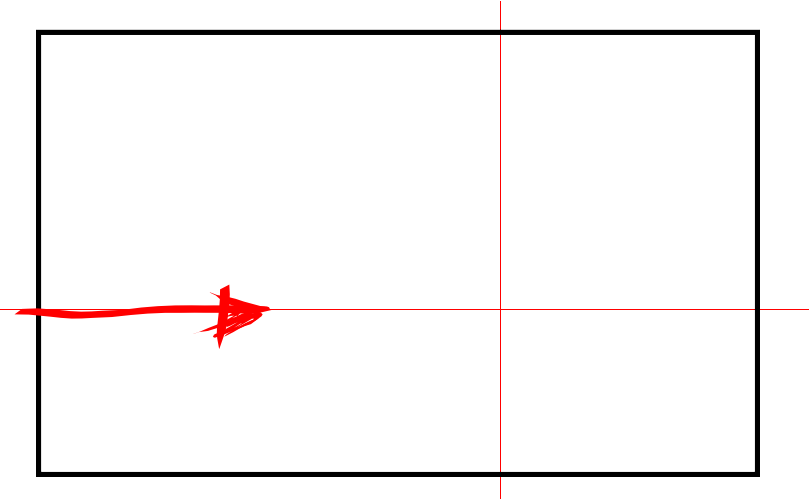
\includegraphics[width=\textwidth]{billeder/scan_direction_right.png}}
    \only<3>{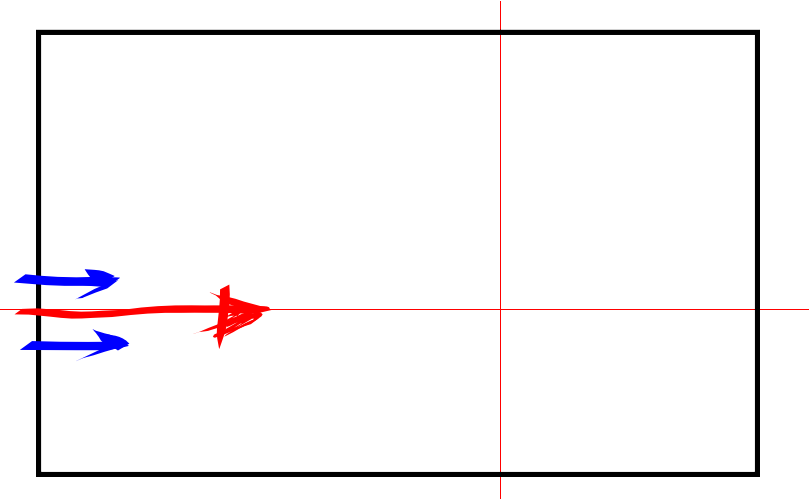
\includegraphics[width=\textwidth]{billeder/scan_direction_right_margin.png}}

\end{frame}

\subsection*{}
\begin{frame}

    \frametitle{Objekter liggende i det gyldne snit}

    To forskellige måder, at betragte en region liggende i et snit på:

    \begin{center}
        \rowcolors[]{1}{blue!20}{blue!10}
        \begin{tabular}{l|cc}
            & Positiv & Negativ\\\hline
            Naiv    & 
\includegraphics[width=0.18\textwidth]{pnaiv_nudvidet} & 
\includegraphics[width=0.18\textwidth]{pudvidet_nnaiv}\\
            Udvidet & 
\includegraphics[width=0.18\textwidth]{pudvidet_nnaiv} & 
\includegraphics[width=0.18\textwidth]{pnaiv_nudvidet}
        \end{tabular}
    \end{center}

\end{frame}

\section{Malerier}
\subsection*{}
\begin{frame}

    \frametitle{Malerier}

    Malerier, sorteret efter rækkefølge i præsentationen

    \begin{itemize}
        \item \emph{Calumny of Apelles} -- Sandro Botticelli -- 1494--95
    \end{itemize}


\end{frame}

\begin{frame}

    \frametitle{Tak}

\end{frame}

\end{document}
